\documentclass[aspectratio=169,10pt]{beamer}
\usetheme{metropolis}
\metroset{block=fill, sectionpage=progressbar}
\setbeamersize{text margin left=0.7cm, text margin right=0.7cm}
\usepackage{fontspec}
\setmainfont{Noto Serif CJK KR}
\setsansfont{Noto Sans CJK KR}
\setmonofont{DejaVu Sans Mono}
\usepackage{amsmath, amssymb}
\usepackage{tikz}
\usetikzlibrary{positioning, arrows.meta, shapes.geometric, fit, backgrounds, calc}
\usepackage{booktabs}
\usepackage{xcolor}

\definecolor{aprlblue}{HTML}{1F4E79}
\definecolor{aprllight}{HTML}{4A7FB5}
\definecolor{aprlaccent}{HTML}{D9531E}
\definecolor{aprlgray}{HTML}{4A4A4A}
\definecolor{aprlbg}{HTML}{F2F4F7}

\setbeamercolor{frametitle}{bg=aprlblue, fg=white}
\setbeamercolor{title separator}{fg=aprlaccent}
\setbeamercolor{progress bar}{fg=aprlaccent, bg=aprlbg}
\setbeamercolor{alerted text}{fg=aprlaccent}

\title{Vision-Language-Action 모델}
\subtitle{RT2에서 $\pi_0$까지, 그리고 그 너머}
\author{Giseop Kim}
\institute{APRL, DGIST \quad $\cdot$ \quad RT604 Spring 2026}
\date{}

\begin{document}

{
\setbeamertemplate{footline}{}
\begin{frame}[plain]
\vspace*{1.5cm}
\begin{center}
{\LARGE\textbf{Vision-Language-Action 모델}}\\[0.3cm]
{\large RT2에서 $\pi_0$까지, 그리고 그 너머}\\[1.5cm]
\textbf{Giseop Kim}\\[0.2cm]
{\small APRL, DGIST}\\[0.1cm]
{\small RT604 \textperiodcentered{} Spring 2026}
\end{center}
\end{frame}
}

% ============================================================
\begin{frame}{오늘 다룰 것}
\begin{enumerate}
  \item \textbf{왜 VLA인가}: 2023년 Coke can 데모가 정말로 의미한 것
  \item \textbf{Google의 길}: SayCan $\to$ RT1 $\to$ PaLM-E $\to$ RT2
  \item \textbf{$\pi_0$ 아키텍처}: PaliGemma + Action Expert
  \item \textbf{내부 동작}: Attention head가 ``pen''을 어떻게 찾는가
  \item \textbf{Flow Matching}: 이미지 생성과 로봇 제어의 통합
  \item \textbf{모델 결합 트릭}: KV cache를 통한 LLM-Expert 공유
  \item \textbf{비판과 대안}: World model 패러다임 (LeCun의 시각)
\end{enumerate}

\vspace{1em}
\footnotesize
\textit{전제 지식}: Transformer, attention, embedding, softmax, diffusion 기초
\end{frame}

% ============================================================
\section{Part 1. Coke Can과 Taylor Swift}

\begin{frame}{2023년 7월: 어색했지만 결정적인 데모}
\begin{columns}[T]
\begin{column}{0.55\textwidth}
\textbf{셋업}
\begin{itemize}
  \item Google 연구실의 책상
  \item Coke can 1개
  \item Tom Cruise, Snoop Dogg, Taylor Swift 사진
\end{itemize}

\vspace{0.5em}
\textbf{명령}
\begin{center}
\textit{``Move the Coke can to Taylor Swift''}
\end{center}

\vspace{0.5em}
\textbf{실행}
\begin{itemize}
  \item RT2는 너무 커서 로봇에 못 올림
  \item 카메라 $\to$ TPU 클러스터 $\to$ 제어 신호
  \item 천천히, 어색하게 사진 가장자리에 올림
\end{itemize}
\end{column}
\begin{column}{0.45\textwidth}
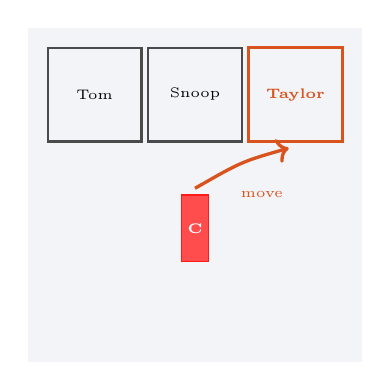
\begin{tikzpicture}[scale=0.85]
\fill[aprlbg] (0,0) rectangle (5,5);
\draw[thick, aprlgray] (0.3,3.3) rectangle (1.7,4.7);
\node at (1,4) {\tiny Tom};
\draw[thick, aprlgray] (1.8,3.3) rectangle (3.2,4.7);
\node at (2.5,4) {\tiny Snoop};
\draw[thick, aprlaccent, line width=1pt] (3.3,3.3) rectangle (4.7,4.7);
\node[aprlaccent] at (4,4) {\tiny\textbf{Taylor}};
\draw[fill=red!70, draw=red!90] (2.3,1.5) rectangle (2.7,2.5);
\node at (2.5,2) {\tiny\textcolor{white}{\textbf{C}}};
\draw[->, very thick, aprlaccent] (2.5,2.6) .. controls (3.2,3) .. (3.9,3.2);
\node[aprlaccent, font=\tiny] at (3.5,2.5) {move};
\end{tikzpicture}

\vspace{0.5em}
\centering\footnotesize
\textit{Carol Houseman: ``이게 정말 될 거라는 \\ 확신이 든 순간이었다.''}
\end{column}
\end{columns}
\end{frame}

% ============================================================
\begin{frame}{왜 이 \textit{어색한} 데모가 돌파구였나}
\textbf{핵심 관찰}: 학습 데이터에 Taylor Swift는 \emph{단 한 번도 등장하지 않았다.}

\vspace{0.5em}
모델이 이 명령을 수행하려면, 두 종류의 지식을 \alert{연결}해야 했다:

\vspace{0.3em}
\begin{columns}[T]
\begin{column}{0.48\textwidth}
\textbf{(A) 인터넷 사전학습}
\begin{itemize}
  \item ``Taylor Swift는 사람이다''
  \item ``이 얼굴이 Taylor Swift다''
  \item 추상적 개념, 의미 관계
\end{itemize}
\end{column}
\begin{column}{0.48\textwidth}
\textbf{(B) 로봇 제어 시연}
\begin{itemize}
  \item ``물체 A를 위치 B로''
  \item gripper 궤적, 힘 제어
  \item physical grounding
\end{itemize}
\end{column}
\end{columns}

\vspace{0.6em}
\begin{block}{함의}
LLM이 \alert{인터넷의 모든 지식}을 \alert{실제 행동}과 연결하는 방법을 학습할 수 있다는 \textbf{최초의 정량적 증거}.
\end{block}

\vspace{0.3em}
\footnotesize
이후 1년 내 RT2 핵심 멤버들이 Google을 나와 \textbf{Physical Intelligence} 창업.
\end{frame}

% ============================================================
\section{Part 2. Google의 진화 경로}

\begin{frame}{2022: SayCan --- LLM을 플래너로}
\begin{columns}[T]
\begin{column}{0.55\textwidth}
\textbf{아이디어}: LLM이 자연어로 task를 \\ subtask로 분해

\vspace{0.6em}
\textbf{예시}: ``엎질러진 것을 닦아라''
\begin{enumerate}
  \footnotesize
  \item 스펀지를 찾는다
  \item 스펀지를 집는다
  \item 엎질러진 곳으로 간다
  \item 닦는다
\end{enumerate}

\vspace{0.6em}
\textbf{한계}
\begin{itemize}
  \item 제어는 \emph{별도}의 imitation network
  \item LLM은 \alert{미리 정해진 메뉴}에서만 선택
  \item 새 객체/장면은 재학습 필요
\end{itemize}
\end{column}
\begin{column}{0.45\textwidth}
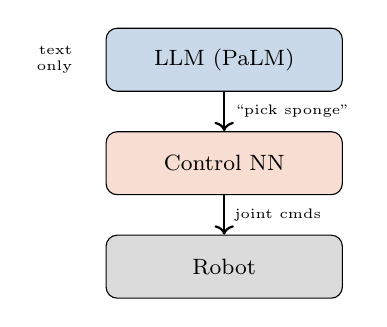
\begin{tikzpicture}[node distance=0.5cm, font=\footnotesize]
\node[draw, rounded corners, fill=aprllight!30, minimum width=3cm, minimum height=0.8cm] (llm) {LLM (PaLM)};
\node[draw, rounded corners, fill=aprlaccent!20, below=of llm, minimum width=3cm, minimum height=0.8cm] (ctrl) {Control NN};
\node[draw, rounded corners, fill=aprlgray!20, below=of ctrl, minimum width=3cm, minimum height=0.8cm] (robot) {Robot};
\draw[->, thick] (llm) -- node[right]{\tiny ``pick sponge''} (ctrl);
\draw[->, thick] (ctrl) -- node[right]{\tiny joint cmds} (robot);
\node[left=0.3cm of llm, font=\tiny, align=right] {text\\only};
\end{tikzpicture}

\vspace{0.5em}
\centering\footnotesize
\textit{LLM이 ``눈을 감은 채'' \\ 계획을 세움}
\end{column}
\end{columns}
\end{frame}

% ============================================================
\begin{frame}{2022 말: RT1 --- 더 큰 행동 메뉴}
\textbf{Robot Transformer 1}
\begin{itemize}
  \item Imitation learning, 그러나 \textbf{대규모}
  \item \alert{130{,}000+ 인간 시연} 데이터셋
  \item Transformer 기반 아키텍처
  \item 입력: 카메라 이미지 + 언어 지시
  \item 출력: 로봇 제어 신호 (joint/gripper)
\end{itemize}

\vspace{0.4em}
\textbf{효과}: SayCan의 LLM 플래너에 \textbf{훨씬 풍부한 메뉴} 제공
\begin{itemize}
  \item Long-horizon 작업 성능 크게 향상
  \item 처음 보는 주방에서 특정 물건 찾기 가능
\end{itemize}

\vspace{0.4em}
\begin{alertblock}{여전한 문제}
플래너 LLM은 \textbf{여전히 텍스트 전용}. 시각 정보 없이 ``눈먼 채'' 계획.
\end{alertblock}
\end{frame}

% ============================================================
\begin{frame}{2023년 3월: PaLM-E --- 시각을 가진 플래너}
\textbf{한 줄 요약}: PaLM에 이미지 입력을 직접 통합한 멀티모달 LLM

\vspace{0.6em}
\textbf{새로 가능해진 것}
\begin{itemize}
  \item 적응형 플래닝: 원하는 물체에 닿으려 다른 물체를 옮김
  \item 자율 회복: 누가 칩 봉지를 다시 서랍에 넣어도 즉시 인식하고 재계획
\end{itemize}

\vspace{0.8em}
\textbf{스택의 형태}: PaLM-E (플래너) + RT1 (제어)

\vspace{0.5em}
\begin{center}
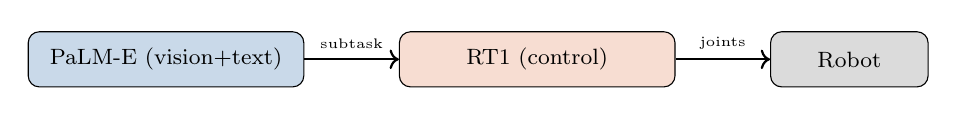
\begin{tikzpicture}[node distance=0.6cm, font=\footnotesize]
\node[draw, rounded corners, fill=aprllight!30, minimum width=3.5cm, minimum height=0.7cm] (palme) {PaLM-E (vision+text)};
\node[draw, rounded corners, fill=aprlaccent!20, right=1.2cm of palme, minimum width=3.5cm, minimum height=0.7cm] (rt1) {RT1 (control)};
\node[draw, rounded corners, fill=aprlgray!20, right=1.2cm of rt1, minimum width=2cm, minimum height=0.7cm] (robot) {Robot};
\draw[->, thick] (palme) -- node[above, font=\tiny]{subtask} (rt1);
\draw[->, thick] (rt1) -- node[above, font=\tiny]{joints} (robot);
\end{tikzpicture}
\end{center}
\end{frame}

% ============================================================
\begin{frame}{관찰: 두 모델이 너무 닮았다}
\begin{columns}[T]
\begin{column}{0.48\textwidth}
\textbf{PaLM-E}
\begin{itemize}
  \item Vision encoder
  \item Transformer
  \item 출력: \textbf{텍스트}
  \item 학습: 다음 토큰 예측, 캡셔닝, task 분해
\end{itemize}
\end{column}
\begin{column}{0.48\textwidth}
\textbf{RT1}
\begin{itemize}
  \item Vision encoder
  \item Transformer
  \item 출력: \textbf{제어 신호}
  \item 학습: 인간 시연 모방
\end{itemize}
\end{column}
\end{columns}

\vspace{1em}
\begin{block}{자연스러운 질문}
PaLM의 출력 vocabulary에 \textbf{action token}을 추가해서, \\
하나의 모델이 텍스트도 행동도 출력하면 어떨까?
\end{block}

\vspace{0.6em}
\centering\textit{즉, LLM이 곧 로봇 두뇌가 될 수 있는가?}
\end{frame}

% ============================================================
\begin{frame}{2023년 7월: RT2 --- 통합의 탄생}
\textbf{레시피}
\begin{enumerate}
  \item PaLM-E와 PaLI-X(또 다른 멀티모달 LLM)에서 출발
  \item RT1과 \emph{동일한} 인간 시연 데이터로 fine-tune
  \item 단, 출력을 \alert{토큰화된 제어 신호}로 변환해 학습
\end{enumerate}

\vspace{0.6em}
\textbf{결과}: 학습 데이터에 없던 객체/장면/지시에 \textbf{일반화}

\vspace{0.6em}
\begin{block}{새로운 패러다임의 이름}
\centering
\Large\textbf{Vision--Language--Action (VLA)}\\
\normalsize Vision $+$ Language $+$ Action $=$ 단일 통합 모델
\end{block}

\vspace{0.5em}
\footnotesize
RT2 모델군: 5B $\sim$ 55B 파라미터. \\
크기 때문에 로봇에서 직접 구동 불가 $\to$ 클라우드 추론 필요.
\end{frame}

% ============================================================
\section{Part 3. $\pi_0$ 아키텍처 해부}

\begin{frame}{2024년 10월: $\pi_0$ --- 더 작고, 더 빠르고, 더 잘하는}
\textbf{Physical Intelligence가 RT2 대비 보여준 도약}
\begin{itemize}
  \item 빨래 개기, 식탁 정리, 그릴드 치즈, 커피, 오렌지 까기, 자물쇠 열기
  \item 처음 보는 침실/주방까지 일반화
\end{itemize}

\vspace{0.8em}
\textbf{놀라운 점: 모델이 더 \textit{작아}졌다}
\begin{center}
\begin{tabular}{lcc}
\toprule
 & RT2 & $\pi_0$ \\
\midrule
파라미터 수 & 5B--55B & \alert{3.3B} \\
구동 환경 & TPU 클러스터 & \alert{RTX 4090 (on-board)} \\
추론 시간 & --- & \alert{73 ms} \\
\bottomrule
\end{tabular}
\end{center}

\vspace{0.8em}
\textbf{질문}: 어떻게 작아지면서도 더 잘하게 만들었는가?
\end{frame}

% ============================================================
\begin{frame}{$\pi_0$ 전체 구조}
\begin{center}
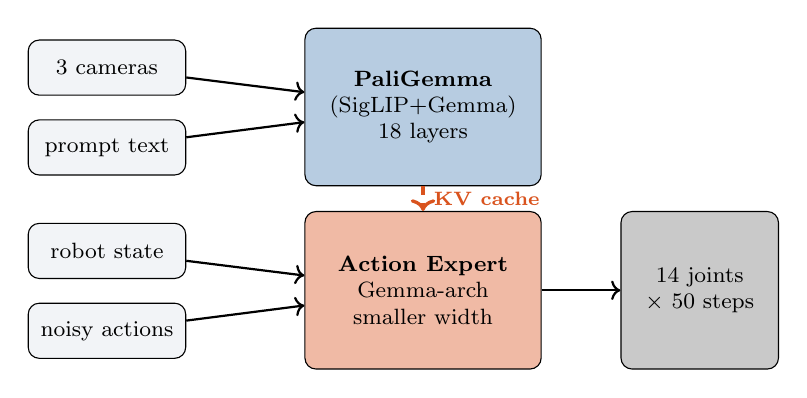
\begin{tikzpicture}[font=\footnotesize, node distance=0.5cm]

% Inputs
\node[draw, fill=aprlbg, rounded corners, minimum width=2cm, minimum height=0.7cm] (img) {3 cameras};
\node[draw, fill=aprlbg, rounded corners, below=0.3cm of img, minimum width=2cm, minimum height=0.7cm] (txt) {prompt text};
\node[draw, fill=aprlbg, rounded corners, below=0.6cm of txt, minimum width=2cm, minimum height=0.7cm] (state) {robot state};
\node[draw, fill=aprlbg, rounded corners, below=0.3cm of state, minimum width=2cm, minimum height=0.7cm] (noise) {noisy actions};

% PaliGemma
\node[draw, fill=aprllight!40, rounded corners, right=1.5cm of img, minimum width=3cm, minimum height=2.0cm, align=center, yshift=-0.5cm] (pg) {\textbf{PaliGemma}\\(SigLIP+Gemma)\\\footnotesize 18 layers};

% Action expert
\node[draw, fill=aprlaccent!40, rounded corners, right=1.5cm of state, minimum width=3cm, minimum height=2.0cm, align=center, yshift=-0.5cm] (ae) {\textbf{Action Expert}\\\footnotesize Gemma-arch\\smaller width};

% Output
\node[draw, fill=aprlgray!30, rounded corners, right=1.0cm of ae, minimum width=2cm, minimum height=2cm, align=center] (out) {14 joints\\$\times$ 50 steps};

% Arrows
\draw[->, thick] (img) -- (pg);
\draw[->, thick] (txt) -- (pg);
\draw[->, thick] (state) -- (ae);
\draw[->, thick] (noise) -- (ae);
\draw[->, thick] (ae) -- (out);

% KV cache sharing - the key insight
\draw[->, very thick, aprlaccent, dashed] (pg.south) -- node[right, font=\scriptsize, aprlaccent]{\textbf{KV cache}} (ae.north);

\end{tikzpicture}
\end{center}

\vspace{0.5em}
\textbf{핵심 설계 결정 3가지}
\begin{enumerate}
  \footnotesize
  \item PaliGemma 백본 + 별도 \textbf{Action Expert} 모듈
  \item Action Expert는 \textbf{flow matching}으로 행동 생성
  \item 두 모듈은 \textbf{KV cache 공유}로 매끄럽게 결합
\end{enumerate}
\end{frame}

% ============================================================
\begin{frame}{설계 결정 1: 왜 Action Expert를 따로 두는가}
RT2 방식: LLM이 \emph{직접} action token 출력

\vspace{0.4em}
$\pi_0$ 방식: Gemma는 ``인지''에, 별도 expert는 ``운동''에 특화

\vspace{0.8em}
\textbf{Action Expert의 정체}
\begin{itemize}
  \item Gemma와 \alert{동일한 아키텍처} (실제 코드에서도 Gemma 클래스로 인스턴스화)
  \item 차이점 1: \textbf{무작위 초기화} (사전학습 없음)
  \item 차이점 2: 각 layer의 \textbf{width가 더 작음} (연산량 감소)
\end{itemize}

\vspace{0.8em}
\begin{block}{SayCan과의 차이 --- 매우 중요}
SayCan: 두 모듈이 \textbf{자연어}로 통신 (저대역폭)\\
$\pi_0$: 두 모듈이 \textbf{attention 내부 표현}으로 통신 (고대역폭)\\
$\Rightarrow$ 사실상 ``하나의 두뇌처럼'' 사고하면서도 모듈성을 유지
\end{block}
\end{frame}

% ============================================================
\section{Part 4. 내부 동작: Attention head}

\begin{frame}{Gemma LLM이 받는 입력}
\textbf{이미지 처리}
\begin{itemize}
  \item 카메라 3대 (overhead + 양쪽 wrist)
  \item 각 이미지 $\to$ 256 patch $\to$ 총 \textbf{768 patches}
  \item Image encoder $\to$ 각 patch당 길이 2048짜리 \textbf{embedding vector}
\end{itemize}

\vspace{0.5em}
\textbf{텍스트 처리}
\begin{itemize}
  \item ``uncap the pen'' $\to$ 4 토큰 $\to$ 4 임베딩 벡터
\end{itemize}

\vspace{0.5em}
\textbf{총합}: $768 + 4 = $ \alert{772 soft tokens}

\vspace{0.8em}
\textbf{Gemma 구조}
\begin{itemize}
  \item 18 transformer blocks
  \item 각 block: attention (8 heads) + MLP
\end{itemize}
\end{frame}

% ============================================================
\begin{frame}{Attention head 한 개의 연산}
입력: 772개의 임베딩 벡터 행렬 $X \in \mathbb{R}^{772 \times d}$

\vspace{0.5em}
\textbf{세 행렬 생성}
\[
Q = X W_Q, \quad K = X W_K, \quad V = X W_V
\]
각각 $772$개의 행 $\Rightarrow$ 입력 토큰 하나당 query/key/value 한 개씩.

\vspace{0.8em}
\textbf{Attention 패턴}
\[
A = \mathrm{softmax}\!\left(\frac{Q K^\top}{\sqrt{d_k}}\right) \in \mathbb{R}^{772 \times 772}
\]

\textbf{출력}
\[
\mathrm{head}(X) = A V \in \mathbb{R}^{772 \times d_v}
\]

\vspace{0.5em}
\footnotesize
직관: 각 query는 ``나에게 관련된 정보가 어디 있나?''를 묻고,\\
$AV$ 곱은 ``그 위치의 value를 내 자리에 가져온다''를 수행.
\end{frame}

% ============================================================
\begin{frame}{사례 연구: ``pen'' 토큰이 펜을 찾는다}
\textbf{시나리오}: 프롬프트의 마지막 토큰 ``pen''의 query 벡터 $q_{\text{pen}}$

\vspace{0.3em}
\textbf{관찰된 행동}
\begin{enumerate}
  \item $q_{\text{pen}}$과 768개 image patch key 사이 dot product
  \item \alert{압도적으로 큰 값}이 \textbf{펜이 보이는 두 patch}에서 발생
  \item Softmax 후 attention map을 이미지에 입히면 \textbf{펜만 빛난다}
\end{enumerate}

\vspace{0.3em}
\begin{center}
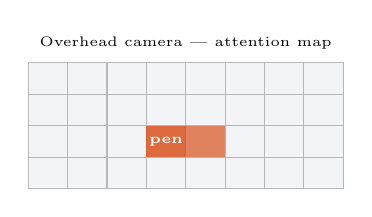
\begin{tikzpicture}[font=\scriptsize]
\fill[aprlbg] (0,0) rectangle (4,1.6);
\foreach \x in {0,0.5,1,1.5,2,2.5,3,3.5} {
  \foreach \y in {0,0.4,0.8,1.2} {
    \draw[aprlgray!40] (\x,\y) rectangle (\x+0.5,\y+0.4);
  }
}
\fill[aprlaccent, opacity=0.85] (1.5,0.4) rectangle (2,0.8);
\fill[aprlaccent, opacity=0.7] (2,0.4) rectangle (2.5,0.8);
\node[font=\tiny] at (2,1.85) {Overhead camera --- attention map};
\node[font=\tiny, white] at (1.75, 0.6) {\textbf{pen}};
\end{tikzpicture}
\end{center}

\vspace{0.2em}
\footnotesize $\Rightarrow$ 모든 프레임에서 \textbf{펜을 자동 추적}. 이것은 18 layer $\times$ 8 head 중 \textbf{단 한 head}의 동작.
\end{frame}

% ============================================================
\begin{frame}{Attention head의 의미론적 해석}
\textbf{$AV$ 곱이 실제로 하는 일}

\vspace{0.5em}
큰 attention 값 $a_{ij}$가 있을 때:
\[
\mathrm{output}_i \mathrel{+}= a_{ij} \cdot v_j
\]
즉, ``pen'' 토큰 위치 $i$에 \textbf{펜 patch} 위치 $j$의 value 벡터가 \alert{복사}되어 더해짐.

\vspace{0.8em}
\begin{block}{한 줄 해석}
이 attention head는 텍스트의 ``pen''과 이미지 속 펜을 \textbf{하나의 통합 표현}으로 묶는다.
\end{block}

\vspace{0.6em}
\textbf{전체 그림}
\begin{itemize}
  \item 18 layer $\times$ 8 head = \textbf{144개의 attention head}
  \item 각 head가 다른 종류의 패턴을 학습
  \item 객체 위치, 손-물체 관계, 시간적 일관성, 작업 진행도 등
\end{itemize}
\end{frame}

% ============================================================
\section{Part 5. Action Expert와 Flow Matching}

\begin{frame}{Action Expert의 입력}
\textbf{입력 1: 로봇 상태 (1 token)}
\begin{itemize}
  \item Aloha 플랫폼: 팔당 7 joint $\times$ 2 = \textbf{14차원 벡터}
  \item Waist, shoulder, elbow, forearm rot, wrist, wrist rot, gripper
  \item $14 \times 1024$ 가중치 행렬로 길이 \alert{1024} embedding으로 매핑
\end{itemize}

\vspace{0.8em}
\textbf{입력 2: 노이즈가 섞인 미래 행동 (50 tokens)}
\begin{itemize}
  \item 다음 50 시간 단계의 14차원 joint 위치 예측
  \item \alert{초기에는 순수 노이즈}로 시작
\end{itemize}

\vspace{0.8em}
\textbf{총 51 tokens} (Gemma의 2048 대비 \textbf{1024}로 축소된 차원 사용)

\vspace{0.4em}
\footnotesize
$\Rightarrow$ Action expert는 가벼움. 그래서 여러 번 반복 실행 가능.
\end{frame}

% ============================================================
\begin{frame}{Flow Matching: 노이즈에서 궤적으로}
\textbf{직관}: 이미지 생성에서 ``노이즈 $\to$ 고양이 사진''하는 것처럼,\\
``노이즈 $\to$ 14$\times$50 관절 궤적''을 만든다.

\vspace{0.6em}
\textbf{왜 잘 작동하는가? 분포가 \alert{multimodal}이기 때문}
\begin{itemize}
  \item 고양이를 그리는 방법은 여러 가지
  \item 펜 뚜껑을 여는 방법도 여러 가지 (어느 손, 어느 각도, 어느 속도)
  \item Single-mode regression은 평균(\textit{mode collapse})을 학습 $\to$ 어색한 동작
\end{itemize}

\vspace{0.6em}
\textbf{$\pi_0$의 절차}
\begin{enumerate}
  \item 무작위 $14\times50$ 행렬 $a^{(0)}$ 생성
  \item Action expert로 update $\Delta a$ 계산
  \item $a^{(t+1)} = a^{(t)} + \Delta a$
  \item \textbf{10번 반복} $\to$ 매끄러운 최종 궤적
\end{enumerate}
\end{frame}

% ============================================================
\begin{frame}{이미지 생성과 로봇 제어의 통합}
\begin{columns}[T]
\begin{column}{0.48\textwidth}
\textbf{이미지 생성}
\begin{itemize}
  \item 입력: 텍스트 + 노이즈 이미지
  \item 출력: 자연 이미지
  \item 분포: 자연 이미지 manifold
\end{itemize}
\vspace{0.3em}
\centering\footnotesize\fbox{noise $\to$ cat}
\end{column}
\begin{column}{0.48\textwidth}
\textbf{로봇 제어 ($\pi_0$)}
\begin{itemize}
  \item 입력: 프롬프트 + 이미지 + 노이즈 궤적
  \item 출력: 14$\times$50 joint 궤적
  \item 분포: 가능한 동작 manifold
\end{itemize}
\vspace{0.3em}
\centering\footnotesize\fbox{noise $\to$ trajectory}
\end{column}
\end{columns}

\vspace{0.8em}
\begin{alertblock}{매우 강력한 추상화}
완전히 다른 응용처럼 보이는 두 영역에서 \textbf{같은 수학적 프레임워크}가 작동한다는 것은 우연이 아닌 \alert{심오한 통일성}.
\end{alertblock}

\vspace{0.4em}
\footnotesize
참고: 이 통찰이 Diffusion Policy, RDT, Octo 등 후속 연구의 토대가 됨.
\end{frame}

% ============================================================
\section{Part 6. 두 모듈의 결합 --- KV cache 트릭}

\begin{frame}{문제 설정}
Action expert도 18 layer $\times$ 8 head를 가진다.

\vspace{0.5em}
\textbf{Action expert의 query는 무엇을 ``보고'' 싶은가?}
\begin{itemize}
  \item 다른 시간 단계의 행동들 (부드러운 궤적을 위해)
  \item \alert{프롬프트} (``무엇을 해야 하는가'')
  \item \alert{이미지} (``펜이 어디 있는가'')
  \item \alert{로봇 상태} (``지금 어디 있는가'')
\end{itemize}

\vspace{0.8em}
\textbf{문제}: 프롬프트와 이미지 정보는 PaliGemma의 attention 안에 있다.\\
어떻게 action expert가 거기에 접근하게 할까?
\end{frame}

% ============================================================
\begin{frame}{해법: Key/Value를 \textit{이어 붙이기}}
\textbf{같은 아키텍처 $\Rightarrow$ 같은 layer index에서 호환}

\vspace{0.3em}
Action expert의 layer $\ell$에서 attention 계산할 때:
\[
K_{\text{total}} = \begin{bmatrix} K^{\text{AE}}_\ell \\ K^{\text{Gemma}}_\ell \end{bmatrix}, \quad
V_{\text{total}} = \begin{bmatrix} V^{\text{AE}}_\ell \\ V^{\text{Gemma}}_\ell \end{bmatrix}
\]
크기: $51 + 772 = $ \alert{823 keys/values}

\vspace{0.4em}
\textbf{Action expert의 query는} 자기 51 token (시간적 일관성)과 Gemma 772 token (의미/시각)을 한 번의 attention으로 \textbf{동시에} 참조 가능.

\vspace{0.4em}
\begin{block}{왜 이게 가능한가}
같은 width, 같은 layer 수, 같은 head 차원 $\Rightarrow$ key/value 공간의 \textbf{차원 호환성}.
\end{block}
\end{frame}

% ============================================================
\begin{frame}{효율성: KV cache 재사용}
\textbf{표준 LLM 추론에서의 KV cache}
\begin{itemize}
  \item 새 토큰이 들어올 때마다 이전 K, V 재계산하지 않고 캐시
\end{itemize}

\vspace{0.6em}
\textbf{$\pi_0$가 영리하게 활용}
\begin{enumerate}
  \item PaliGemma forward pass 1번 $\to$ 모든 layer의 $K^{\text{Gemma}}_\ell, V^{\text{Gemma}}_\ell$ 캐시
  \item Flow matching은 \textbf{10번 반복} 필요
  \item 매 반복마다 \alert{같은 캐시 재사용} (이미지/프롬프트는 안 바뀜)
\end{enumerate}

\vspace{0.6em}
\begin{block}{성능 영향}
이 캐싱 덕분에 \textbf{10회 디노이징}을 \textbf{73 ms}에 끝낼 수 있음.\\
$\Rightarrow$ on-board RTX 4090에서 실시간 제어 가능.
\end{block}
\end{frame}

% ============================================================
\begin{frame}{$\pi_0$의 한 step 전체 흐름}
\begin{enumerate}
  \item 카메라 3장 + 텍스트 프롬프트 + 현재 robot state 수집
  \item PaliGemma forward pass $\to$ 모든 layer의 K/V 캐시
  \item Action expert 초기화: state token + 50개 noise token
  \item \textbf{Flow matching 루프 (10회)}
    \begin{itemize}
      \footnotesize
      \item 각 layer에서 self-attention + cross-attention via concatenated K/V
      \item $\Delta a$ 계산, 궤적 업데이트
    \end{itemize}
  \item 최종 14$\times$50 궤적 출력
  \item 로봇이 처음 몇 step 실행
  \item 새 이미지 받아 1번부터 반복
\end{enumerate}

\vspace{0.6em}
\centering
\textit{73 ms / cycle $\to$ 약 13 Hz 제어 루프}
\end{frame}

% ============================================================
\section{Part 7. 비판적 시각과 미래}

\begin{frame}{데모를 신중히 읽기: 1995년 Ralph}
\textbf{Carnegie Mellon, 1995}
\begin{itemize}
  \item 자율주행 시스템 ``Ralph''
  \item 미국 횡단 \textbf{98.2\% 자율}
\end{itemize}

\vspace{0.6em}
\textbf{30년 후의 자율주행}
\begin{itemize}
  \item Ralph의 직계 후손이 아니다
  \item 센서 융합, HD map, learned planner, end-to-end transformer 등 \textbf{전혀 다른 패러다임}
\end{itemize}

\vspace{0.8em}
\begin{alertblock}{교훈}
인상적인 데모와 ``실제로 작동하는 시스템''은 \textbf{다른 문제}.\\
$\pi_0$도 ``집안일을 다 해주는 로봇''까지는 한참 남았다.
\end{alertblock}
\end{frame}

% ============================================================
\begin{frame}{대안 패러다임: World Models}
\textbf{등장 배경}: VLA가 정말 ``올바른 길''인지에 대한 의문

\vspace{0.3em}
\textbf{Yann LeCun (전 Meta 수석 AI 과학자)}
\begin{itemize}
  \item Meta를 떠나 \textbf{world model 중심} 벤처 창업
  \item LLM 백본을 쓰지 \alert{않는} 방향, JEPA 계열
\end{itemize}

\vspace{0.3em}
\begin{block}{LeCun의 입장 (인용)}
\textit{``VLA are doomed. They basically don't work really well.''}
\end{block}

\vspace{0.3em}
\textbf{핵심 차이}
\begin{itemize}
  \item VLA: 인터넷 텍스트/이미지 사전학습 $\to$ 행동으로 fine-tune
  \item World model: 환경의 \textbf{예측 모델}을 latent space에서 학습
  \item Planning은 학습된 world model 위에서 search/optimization
\end{itemize}
\end{frame}

% ============================================================
\begin{frame}{토론거리 (대학원 수업용)}
\begin{enumerate}
  \item RT2의 일반화 (Taylor Swift)는 진짜 ``이해''인가, 아니면 통계적 보간인가?
  \vspace{0.3em}
  \item Action expert를 따로 두는 것은 \textbf{귀납적 편향}을 주입한 것이다. 이는 ``순수 end-to-end'' 철학과 충돌하는가, 보완하는가?
  \vspace{0.3em}
  \item Flow matching이 mode collapse를 피한다고 했다. 그럼 \textbf{원치 않는 mode} (안전하지 않은 동작)도 학습될 위험은?
  \vspace{0.3em}
  \item KV cache 공유는 ``같은 아키텍처''에 의존한다. \textbf{이종 모듈}을 결합하는 더 일반적인 방법은?
  \vspace{0.3em}
  \item LeCun의 주장이 옳다면, classical SLAM/state estimation의 역할은 미래 로봇 두뇌에서 어떻게 자리잡을까? \\
        \footnotesize\textit{(Hint: APRL의 ``Classical-to-Modern Bridge'' 관점)}
\end{enumerate}
\end{frame}

% ============================================================
\begin{frame}{핵심 정리}
\begin{enumerate}
  \item \textbf{VLA}: Vision + Language + Action을 단일 모델에서 통합
  \vspace{0.2em}
  \item \textbf{$\pi_0$ 설계 3원칙}
    \begin{itemize}
      \footnotesize
      \item 백본 LLM (PaliGemma) + 별도 Action Expert
      \item Flow matching으로 궤적 생성
      \item KV cache 공유로 효율적 모듈 결합
    \end{itemize}
  \vspace{0.2em}
  \item \textbf{이중 통합}
    \begin{itemize}
      \footnotesize
      \item 인터넷 지식 $\leftrightarrow$ 물리적 행동
      \item 이미지 생성 수학 $\leftrightarrow$ 로봇 제어 수학
    \end{itemize}
  \vspace{0.2em}
  \item \textbf{한계와 대안}: World model 패러다임은 다른 길을 제시
  \vspace{0.2em}
  \item \textbf{연구자에게}: 데모와 실제 시스템 사이 간극을 잊지 말 것
\end{enumerate}
\end{frame}

% ============================================================
\begin{frame}{참고 문헌 (시작점)}
\footnotesize
\begin{itemize}
  \item Ahn et al. (2022) ``Do As I Can, Not As I Say: Grounding Language in Robotic Affordances'' (SayCan)
  \item Brohan et al. (2022) ``RT-1: Robotics Transformer for Real-World Control at Scale''
  \item Driess et al. (2023) ``PaLM-E: An Embodied Multimodal Language Model''
  \item Brohan et al. (2023) ``RT-2: Vision-Language-Action Models Transfer Web Knowledge to Robotic Control''
  \item Black et al. (2024) ``$\pi_0$: A Vision-Language-Action Flow Model for General Robot Control''
  \item Beyer et al. (2024) ``PaliGemma: A versatile 3B VLM for transfer''
  \item Lipman et al. (2023) ``Flow Matching for Generative Modeling''
  \item LeCun (2022) ``A Path Towards Autonomous Machine Intelligence'' (JEPA position paper)
\end{itemize}

\vspace{1em}
\centering
\textbf{다음 주}: World model과 JEPA 계열 깊이 다루기
\end{frame}

\end{document}
